\documentclass{article}

\usepackage{mathtools}

\usepackage{tikz}
\usepackage[margin=1in]{geometry}

\title{FCA}
\author{ale-cci}

\begin{document}
\maketitle
\newpage
\section{Criterio di Juri}
Sia dato il polinomio $a(z) = a_n z^n + a_{n-1} z^{n-1} + \cdots + a_n$ con $a_n > 0$. Condizione necessaria affich\'e $a(z)$ abbia tutte le radici di modulo minore di $1$ \'e che le seguenti disuguaglianze siano soddisfatte:

\begin{enumerate}
    \item $a(1) > 0$
    \item $(-1)^n a(-1) > 0$
    \item $|a_0| < a_n$
\end{enumerate}

Perndendo come esempio il caso $n - 1$:
\[ a(z) = a_1z + a_0 = 0 \]
\[ z = -\frac{a_0}{a_1} \qquad |z| < 1 \quad \Leftrightarrow \quad \frac{|a_o|}{a_1} < 1 \quad \Leftrightarrow\quad  \framebox{$|a_o| < a_1$} \]

Otteniamo che:
\begin{itemize}
    \item $ a(1) = a_1 + a_0 > 0$
    \item $ a(-1) = -a_1 + a_0 < 0$
\end{itemize}

di queste tre disuguaglianze solo 2 sono indipendenti: la terza \'e l'insieme della prima e della seconda

Per il caso $n = 2$: 3 condizioni distinte (page 14 di Lez. 21)


\bigbreak
Anche nel criterio di Jury \'e necessario costruire una trabella: (slide 15 Lez 21)
\begin{itemize}
    \item iniziamo a scrivere le prime due righe: con la prima riga iniziamo a scrivere a partire da $a_0$
    \item Per la seconda riga partiamo da $a_n$ e terminiamo la riga a $a_0$
    \item Per costruire le right successive calcoliamo il determinante della matrice $2\times 2$ sopra e riportiamo la stessa riga sotto al contrario
\end{itemize}

Per calcolare il termine di una determinata riga si utilizza la formula:
\[
    b_k = \det\begin{pmatrix}
        a_0 & a_{n-k}\\
        a_n & a_k
    \end{pmatrix} \quad k = 0,1\ldots n-1
\]

\section{Teorema (criterio di Jury)}
Il polinomio $a(z) = \ldots$ ha tutte le radici di modulo minore di 1 se e solo se le seguenti $n+1$ disuguaglianze sono soddisfatte:
\begin{enumerate}
    \item $a(1) > 0$
    \item $(-1)^n a(-1) > 0$
    \item $\ldots$ slide 16
\end{enumerate}

\section{Scelta del periodo di campionamento (Slide 18 Lez 21)}

Per il teorema di campionamento
\[ w_s > 2w_b \]
con $w_s = \frac{2\pi}{}$ pulsazione di campionamento, $T$ il corrispondente periodo

Una volta realizzato il progetto in tempo continuo \'e necessario implementare una $C_d(z)$

Alla funzione $C(s)$ \'e associata un'equazine differenziale in tempo continuo, a $C_d(z)$  un equazione di differenze

Metodo di eulero: $Dx(T) \Rightarrow \mathcal{L}[Dx(t)] = s\cdot\mathcal{L}[x(t)]$ (condizione iniziale nulla)
\[ Dx(kT) \approx \frac{x((k+1)T) - x(kT)}{T}\]
\[ \mathcal{Z}[Dx(kT)]  \approx \frac{z-1}{T}\mathcal{Z}[x(kT)]\]
\[ s = \frac{z-1}{Tz}\]

\subsubsection{Alla lavagna}

Immaginando di avere la funzione differenziale $a_1 Dy + a_0y = b_1Du + b_0u$ corrisponde una funzione di trasferimento.
Trasformandola secondo laplace con, condizioni iniziali nulle si ottiene:

\[ a_1 sY + a_0 Y = b_1 sU + b_0 U \]

Immaginandola in tempo discreto, imponendo $t = kT$
\[ a_1 Dy(kT) + a_0 y(kT_ = b_1 Du(kT) + b_0u(kT) \]

NOTA: Fino ad adesso Non \'e una approssimazione

Ora per calcolare la derivata utilizzo l'euqazione di eulero
\[ a_1 \frac{y((k+1)T) - y(kT)}{T} + a_0 y(kT) = b_1\frac{u((k+1)T) - u(kT)}{T} + b_0u(kT)\]

Trasformanso:
\[ \mathcal{Z}\left\{a_1 \frac{y((k+1)T) - y(kT)}{T} + a_0 y(kT) = b_1\frac{u((k+1)T) - u(kT)}{T} + b_0u(kT)\right\}\]

\[ \cdots\]
\[ a_1 \frac{z-1}{T} \mathcal{Z}[y(kT)] + a_0 \mathcal{Z}[y(kT)] = b_1 \frac{z-1}{T} \mathcal{Z}[u(kT)] + b_0 \mathcal{Z}[u(kT)]\]

Trovo cos\`i che:
\[ Y(z) = \frac{b_1\frac{z-1}{T} + b_0}{a_1\frac{z-1}{T} + a_0} U(z) = \left.C(s)\right|_{s=\frac{z-1}{T}} U(z) \coloneqq H(z)U(z)\]

\bigbreak

\textbf{Metodo di Euolero all'indietro}: Stimo la derivata guardando il campione precedente

\[ Dx(kT) \approx \frac{x(kT) - x((k-1)T)}{T}\]

\subsubsection{Metodo di Tustin (slide 21)}
Viene utilizzata l' `approssimazione col metodo del trapezio'

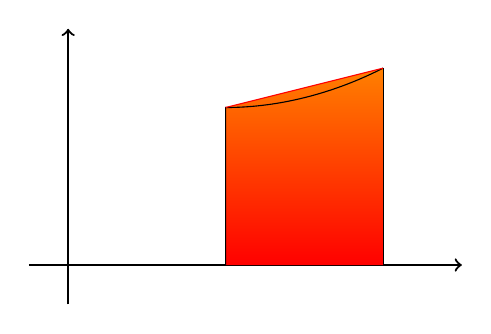
\begin{tikzpicture}
    \draw [thick, ->] (-0.5, 0) -- (5, 0);
    \draw [thick, ->] (0, -0.5) -- (0, 3);
    \shade[top color=orange, bottom color=red] (2, 2) -- (4, 2.5) |- (2, 0);
    \draw (2, 0) -- (2, 2)
            parabola (4, 2.5);
    \draw (4, 0) -- (4, 2.5);

    \draw [color = red] (2, 2) -- (4, 2.5);

\end{tikzpicture}

(x: Approssimare due  punti con trapezio)

Da slide 24: $C_d(z)$ \`e asintoticamente stabile siccome tutti i poli sono contenuti nella circonferenza unitaria






\newpage
\section{Esercizi}
\subsection{Ex Lez 20 Slide 16}

\subsubsection{Parte 1}

\[
    y_0(K+2) = y(K+1) - 0.24y(K) + u(K+2)\\
\]
\bigbreak
\(
    a_ny(K) + a_{N-1}y(K-1) + \cdots +a_o y(K-1) = b_n u(K-n +m) + b_{n-1} u(K-n+m-1) + \cdots + b_o u(K-n)
\)

\(
\Leftrightarrow H(z) = \frac{b_mz^{n} + b_{m-1}z^{m-1}+ \cdots + b_o}{a_mz^n + a_{n-1}z^{n-1}+a_0}
\)
\bigbreak

\(
\begin{cases}
a_n \neq 0\\
b_m \neq 0 \\
m \le n
a_0 \lor b_0 \neq 0
\end{cases}
\)

\[
\begin{split}
K \leftarrow K-1\\
y(K) = y(K-1) - 0.24 y(k-2) + u(K)\\
y(K) - y(K-1) + 0.24 y(K-2) = u(k)
\end{split}
\]

\begin{enumerate}
    \item $K-2 = K - n \Rightarrow n = 2$
    \item $K = K - n + m \Rightarrow 0 = -n + m \qquad m = n = 2$
\end{enumerate}


Grado di relativit\'a $g = m-n = 0$

\begin{align*}
Y(z) = -Z^{-1} Y(z) + 0.24 Z^{-2} Y(z) = U(z)\\
Y(z) \cdot (1-Z^{-1} + 0.24 Z^{-2}) =  U(z)\\
Y(z) = \frac{1}{1-Z-1 + 0.24 Z^{-2}}U(z) = \frac{Z^{-2}}{Z^2 - z + 0.24} U(z)\\
n = 2, m=2 \Rightarrow \rho = n - m = 0
\end{align*}

\subsubsection{Parte 3}
\[
\begin{split}
    Z[ a^{k-1} 1(K-1)] = \frac{1}{z-a}\\
    Z[ (K-1) a^{k-2} 1(K-1)] = \frac{1}{(z-a)^2}\\
    H(z) = Z(h(K)) = \frac{1}{z-1} -
    \frac{5}{2} \frac{1}{\left( z - \frac{1}{2}\right)} - 7 \frac{1}{z-\frac{1}{z - \frac{1}{2}}} = \\
    \cdots = \frac{z^2 +1}{z^3 -2z^2 + \frac{5}{4} z - \frac{1}{4}}
\end{split}
\]
\[
    y(K) - 2y(K-1) + \frac{5}{4}y(K-2) - \frac{1}{4}y(K-3) = u(K-1) + u(K-3)
\]


% Esercizi

\subsubsection{1}

\[ a(z) = z^3 - z^2 + z  0.5 \]
\begin{align*}
    &1.\quad a(1) > 0 \qquad 1 - 1 + 1 + 0.4 = 1.5 > 0 \quad \text{OK}\\
    &2.\quad (-1)^3 a(-1) > 0, a(-1) < 0\\
    & \quad -a(-1) > 0 \qquad -1 -1 -1 +0.5 = -2.5 < 0 \quad \text{OK}\\
    &3.\quad  |a_0| < a_3 \qquad |0.5| < 1 \text{OK!}
\end{align*}

\begin{tabular}{c|c c c c}
    1 & 0.5 & 1&  -1 & 1\\
    2 & 1 & -1 & 2 & 0.5\\
    3 & -0.75 & 1.5 & -1.5\\
    4 & -0.75 & -1.5 & &
\end{tabular}

\bigbreak
$|-0.75| > |-1.5|$ Not OK!

\subsubsection{Secondo esercizio (slide 27)}

\[ a(z) = z^4 - z^3 + 0.25 z^2 + 0.25 z - 0.125 \]

Per calcolare se il sistema \'e asintoticamente stabile

\begin{align*}
    &1.\quad  a(1) > 0! \quad a(1) = 1 -1 + 0.25 + 0.25 - 0.125 = 0.357 > 0 & \text{OK}\\
    &2. \quad (-1) ^4 a(-1) > 0 \\
    & \quad a(-1) > 0 \quad a(-1) = 1 + 1 + 0.25 - 0.25 -0.125 = 1.875 > 0 & \text{OK}\\
    &3 \quad |a_0| < a_4 \quad |-o.125| < 1 & \text{OK} \\
    & 4. \quad |b_0| > |b_1| \qquad |-0.9875| > |-0.125| & \text{OK}\\
    & 5.\quad  |c_0| > |c_2| \qquad |0.9534| > |0.3979| & \text{OK}\\
\end{align*}

\begin{tabular}{c|c c c c c}
    1 & -0.125 & 0.25 & 0.25 & -1 & 1\\
    2 & 1 & -1 & 0.25 & 0.25 & -0.125\\
    \\
    3 & -0.98475 & 0.96875 & -0.28125 & -0.125\\
    4 & -0.125 & -0.28125 & 0.96875 & -0.984375\\
    \\
    5 & 0.9534 & * & 0.3979
\end{tabular}
\end{document}
